\documentclass[letterpaper]{article}
\usepackage[submission]{aaai2027}
\usepackage[hyphens]{url}
\usepackage{graphicx}
\urlstyle{rm}
\def\UrlFont{\rm}
\usepackage{natbib}
\usepackage{caption}
\frenchspacing
\usepackage{booktabs}
\usepackage{amsmath}

\pdfinfo{/TemplateVersion (2027.1)}
\setcounter{secnumdepth}{2}
\renewcommand{\thesection}{S\arabic{section}}
\renewcommand{\thetable}{S\arabic{table}}
\renewcommand{\thefigure}{S\arabic{figure}}

\title{Trajectory-Aligned Latent Handoff for Efficient High-Resolution Video Diffusion\\Supplementary Material}
\author{Anonymous Submission}
\affiliations{}

\begin{document}
\maketitle

\section{Extended Operator Evaluation}

Table~\ref{tab:s_operator} reports the complete paired evaluation of CLL against trilinear latent lifting. Each setting contains 50 samples and uses the VAE encoding of the matched high-resolution video as reference. CLL improves every reported mean at both scale factors. At the more aggressive 368p-to-720p transition, PSNR improves on 37 of 50 samples; the perceptual and temporal metrics provide the more consistent evidence in this setting.

\begin{table*}[t]
\centering
\small
\begin{tabular}{llrrrrr}
\toprule
Input $\rightarrow$ output & Operator & Latent $L_1\downarrow$ & PSNR $\uparrow$ & SSIM $\uparrow$ & LPIPS $\downarrow$ & Temp. $L_1\downarrow$ \\
\midrule
480p $\rightarrow$ 720p & Trilinear & 0.1929 & 24.29 & 0.7159 & 0.2358 & 0.02121 \\
480p $\rightarrow$ 720p & CLL & \textbf{0.0991} & \textbf{30.00} & \textbf{0.8696} & \textbf{0.0629} & \textbf{0.01468} \\
368p $\rightarrow$ 720p & Trilinear & 0.2444 & 23.42 & 0.6740 & 0.3352 & 0.02388 \\
368p $\rightarrow$ 720p & CLL & \textbf{0.1628} & \textbf{24.10} & \textbf{0.7592} & \textbf{0.1640} & \textbf{0.02017} \\
\bottomrule
\end{tabular}
\caption{Operator-level comparison between CLL and trilinear lifting ($n=50$).}
\label{tab:s_operator}
\end{table*}

\section{Trajectory Alignment Statistics}

All final TAA models use alignment intensity 0.75. Table~\ref{tab:s_alignment} reports paired endpoint statistics. The step-45 row is recomputed from the final intensity-0.75 per-sample outputs; it does not use the earlier intensity-1.0 development result. The low-resolution temporal metric measures error relative to the completed low-resolution endpoint and is distinct from the human temporal preference on decoded 720p videos.

\begin{table*}[t]
\centering
\small
\begin{tabular}{lrrrrrr}
\toprule
Trajectory / handoff & Unaligned $L_1\downarrow$ & TAA $L_1\downarrow$ & Reduction & 95\% CI & Win/Loss & $p$ \\
\midrule
Wan50, Steps 40 $\rightarrow$ 50 & 0.03215 & \textbf{0.02385} & 25.82\% & [0.00479, 0.01302] & 10/0 & 0.00195 \\
Wan50, Steps 45 $\rightarrow$ 50 & 0.02363 & \textbf{0.01866} & 21.03\% & [0.00260, 0.00840] & 10/0 & 0.00195 \\
Distill4, Steps 3 $\rightarrow$ 4 & 0.04286 & \textbf{0.04070} & 5.03\% & [0.00148, 0.00299] & 10/0 & 0.00195 \\
\bottomrule
\end{tabular}
\caption{Paired trajectory-alignment results at intensity 0.75.}
\label{tab:s_alignment}
\end{table*}

At step 40, intensities 0.5 and 1.0 improve mean endpoint $L_1$ by only 0.00012 and 0.00071, whereas 0.75 gives the lowest endpoint error, a 10/0 paired win rate, and the highest downstream VBench-5. This non-monotonic response motivates selecting the handoff strength with both endpoint and downstream evaluations.

\section{Extended Qualitative Comparison}

Figure~\ref{fig:s_qualitative} uses fixed frame indices and identical crop coordinates across methods. Native-HR (estimated) is the content-aligned complete 368p trajectory shown at the common display size. It is used for structure and motion reference because native 368p and native 720p sampling can generate different contents under the same prompt and seed; actual 720p Native-HR Sampling remains the quantitative baseline in the main paper.

\begin{figure*}[t]
\centering
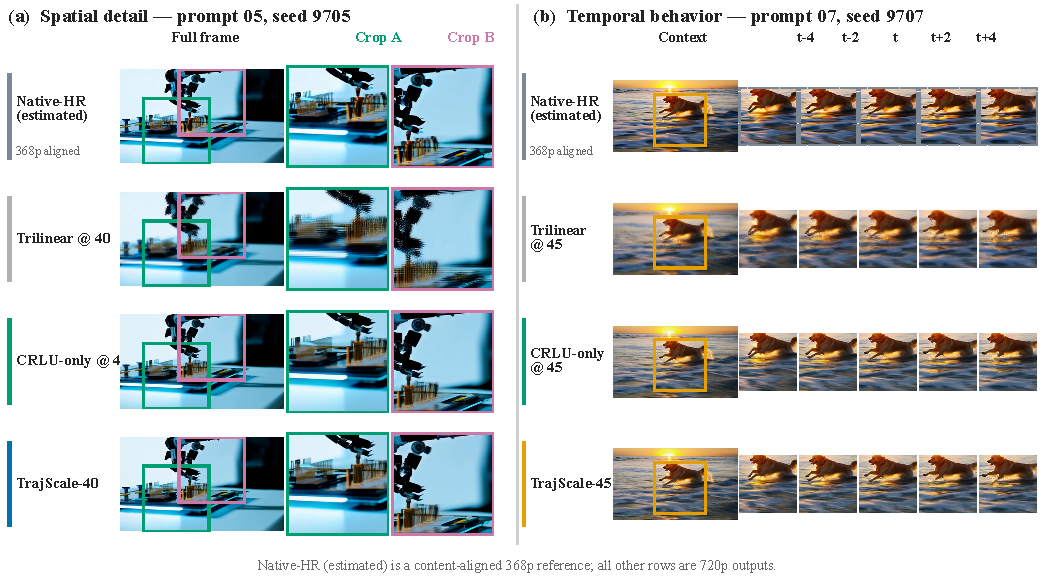
\includegraphics[width=0.90\textwidth]{figures/supplementary/fig_qualitative.pdf}
\caption{Matched real-video frames. The spatial panel compares trilinear lifting, CLL-only handoff, and TALH-Q. The temporal panel uses fixed consecutive frames to expose the detail--temporal behavior of CLL-only and TALH-E.}
\label{fig:s_qualitative}
\end{figure*}

\section{Human Evaluation Details}

Three independent raters viewed randomized, double-blind pairs for each of ten prompts. Prompt-level majority vote is the statistical unit; ties are retained. Table~\ref{tab:s_human} reports the comparisons used in the main text. Two-sided exact sign tests exclude tied prompts.

\begin{table*}[t]
\centering
\small
\begin{tabular}{lrrr}
\toprule
Comparison (former vs. latter) & Details (W/L/T) & Overall (W/L/T) & Temporal (W/L/T) \\
\midrule
TAA vs. Unaligned, both CLL (Step 40) & 8/2/0 & 6/2/2 & 1/9/0 \\
TAA vs. Unaligned, both CLL (Step 45) & \textbf{9/0/1} & \textbf{6/0/4} & 0/8/2 \\
CLL-only vs. Trilinear (Step 45) & \textbf{10/0/0} & \textbf{10/0/0} & \textbf{8/0/2} \\
TALH-E vs. Trilinear (Step 45) & \textbf{10/0/0} & \textbf{10/0/0} & \textbf{9/0/1} \\
\bottomrule
\end{tabular}
\caption{Prompt-level majority votes ($n=10$, three raters per prompt). Bold entries have exact sign-test $p<0.05$.}
\label{tab:s_human}
\end{table*}

For the step-45 TAA-with-CLL comparison, observed agreement/Fleiss' $\kappa$ are 0.733/0.070 for detail, 0.567/0.097 for overall quality, and 0.300/$-0.388$ for temporal stability. For TALH-E versus trilinear handoff, observed agreement is 0.933 for details and overall quality and 0.567 for temporal stability; the corresponding $\kappa$ values are $-0.034$, $-0.034$, and $-0.168$. The low or negative $\kappa$ values coexist with strongly one-sided majority outcomes because expected agreement is also high, a prevalence-sensitive regime. We therefore report both majority counts and agreement rather than interpreting $\kappa$ alone.

\section{Reproducibility Notes}

All 50-step comparisons use matched prompts, seeds, initial noise, scheduler, shift 8, and CFG 6. TALH-Q and TALH-E hand off at evaluations 40 and 45. The four-step sampler uses nominal timesteps $[1000,750,500,250]$, shift 5, and handoff at the third evaluation. CLL and TAA train on four H100 GPUs for approximately 8 and 33 wall-clock hours. Train, validation, and test sets are disjoint in both prompt and seed. The cached-prefix argument applies only to deterministic, condition-matched prefixes with TAA inactive before the handoff.

\end{document}
